\documentclass[conference]{IEEEtran}
\IEEEoverridecommandlockouts
% The preceding line is only needed to identify funding in the first footnote. If that is unneeded, please comment it out.

\usepackage{amsmath,amssymb,amsfonts}
\usepackage{algorithmic}
\usepackage{graphicx}
\usepackage{textcomp}
\usepackage{xcolor}
\usepackage{natbib}
\usepackage{stfloats}
\usepackage{booktabs}
\usepackage{multirow}
\usepackage{microtype}
\usepackage{titlesec}
\usepackage{placeins}
\usepackage{hyperref}
% \bibliographystyle{abbrv}

\usepackage{caption}
\captionsetup[table]{
  position=below,
  labelformat=simple,
  labelsep=colon,
  font=footnotesize,
  labelfont={footnotesize,bf},
  textfont={footnotesize,normalfont},
  justification=justified,
  singlelinecheck=false
}
\renewcommand{\thetable}{\arabic{table}}

\titlespacing*{\section}{0pt}{2.2ex plus 0.6ex minus 0.2ex}{1.1ex plus 0.2ex}
\titlespacing*{\subsection}{0pt}{1.7ex plus 0.5ex minus 0.2ex}{0.8ex plus 0.2ex}
\titlespacing*{\subsubsection}{0pt}{1.4ex plus 0.4ex minus 0.2ex}{0.6ex plus 0.2ex}

\setlength{\textfloatsep}{12pt plus 2pt minus 2pt}
\setlength{\floatsep}{10pt plus 2pt minus 2pt}
\setlength{\intextsep}{10pt plus 2pt minus 2pt}
\setlength{\abovedisplayskip}{8pt plus 2pt minus 2pt}
\setlength{\belowdisplayskip}{8pt plus 2pt minus 2pt}
\setlength{\abovedisplayshortskip}{6pt plus 2pt minus 2pt}
\setlength{\belowdisplayshortskip}{6pt plus 2pt minus 2pt}



\def\BibTeX{{\rm B\kern-.05em{\sc i\kern-.025em b}\kern-.08em
    T\kern-.1667em\lower.7ex\hbox{E}\kern-.125emX}}
\begin{document}

\title{CortexDecoder: fMRI-to-image Reconstruction from Cortical Flatmaps
\\
{\footnotesize \textsuperscript{}}
% \thanks{Identify applicable funding agency here. If none, delete this.}
}

\author{
\IEEEauthorblockN{Teo Imoto-Tar\IEEEauthorrefmark{1}}
\IEEEauthorblockA{\textit{Department of Mathematics} \\
\textit{University of California, San Diego}\\
timototar@ucsd.edu}
\and
\IEEEauthorblockN{Maxwell Fung\IEEEauthorrefmark{1}}
\IEEEauthorblockA{\textit{College of Computing, Data Science, and Society} \\
\textit{University of California, Berkeley}\\
maxwellfung@berkeley.edu}
\and
\IEEEauthorblockN{Arnav Gurha}
\IEEEauthorblockA{\textit{School of Biological Sciences} \\
\textit{University of California, San Diego}\\
agurha@ucsd.edu}
% \thanks{\IEEEauthorrefmark{1}These authors contributed equally to this work.}
% \and
% \IEEEauthorblockN{Nikaash Bahl}
% \IEEEauthorblockA{\textit{Department of Bioengineering} \\
% \textit{University of California San Diego}\\
% nibahl@ucsd.edu}
}

\makeatletter
\twocolumn[
  \begin{@twocolumnfalse}
    \maketitle
    \begin{center}
      \resizebox{\textwidth}{!}{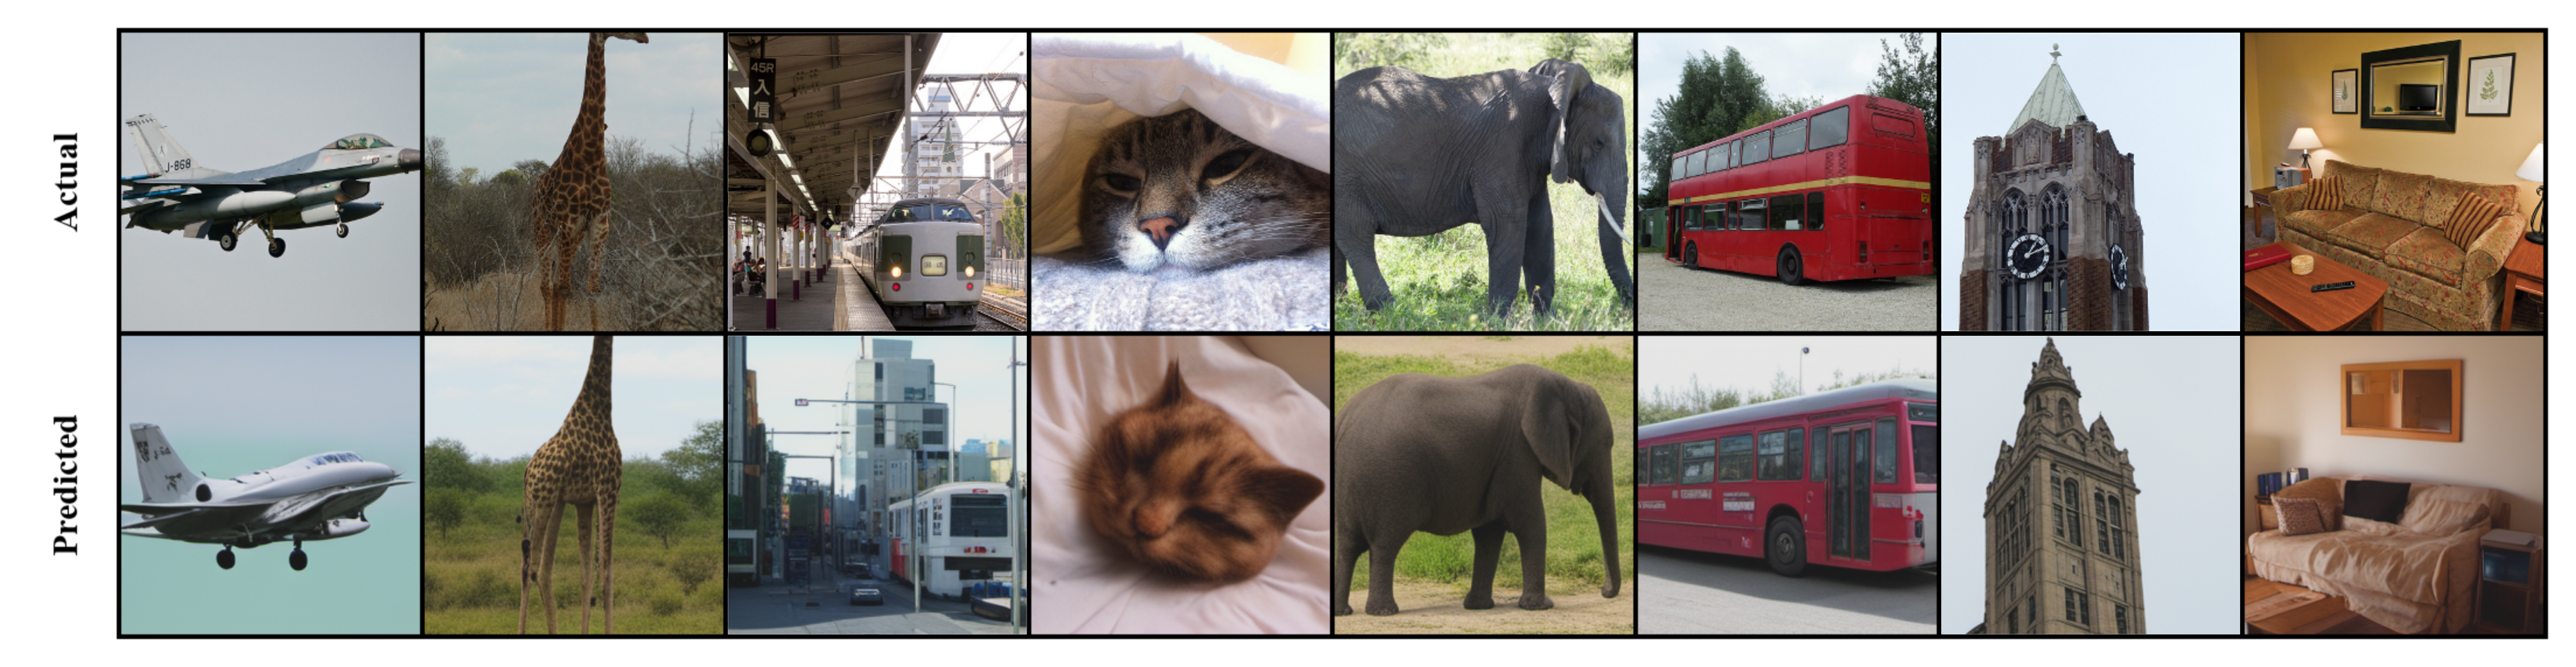
\includegraphics{images/title3.png}}
      \captionof{figure}{Collage of CortexDecoder predictions on the bottom row and the original image stimuli on the top row. Images including those depicting faces are derived from the Microsoft COCO dataset, used under CC BY 4.0. \cite{lin2015microsoftcococommonobjects}}
      \label{fig:title}
    \end{center}
    \vspace{1em}
  \end{@twocolumnfalse}
]
\makeatother

\begin{abstract}
Recent advances in brain decoding work has shown the potential of Vision Transformers (ViTs) to learn mappings from neural representation to visual features. Here we present CortexDecoder, a brain decoding framework mapping fMRI flatmaps to images viewed by subjects. Flatmaps are neural responses projected onto cortical surfaces and then unfolded into 2D images. We demonstrate that (1) flatmaps preserve sufficient signal to achieve high performance in brain decoding; raw fMRI data has noisy signals and high-dimensionality which makes decoding a difficult task. (2) Reshaping raw fMRI data into flatmaps allows for clean patch-based tokenization. This allows us to harness state-of-the-art Vision Transformers to learn meaningful neural representations and preserve spatial encoding. To do this, we pass flatmap patches into a pretrained CortexMAE encoder to obtain brain tokens. A lightweight cross-attention bridge then learns to map these brain tokens to image features. Our cross-attention bridge is split into two modules; the semantic module for predicting CLIP embeddings and the lower-level module to generate low-level image reconstruction. Finally, a fine-tuned SDXL (Stable Diffusion XL) takes this low-level reconstruction image as the initial image. Conditioned by the CLIP semantic embedding, the SDXL produces the final reconstruction image. In single-subject evaluations, CortexDecoder achieves performance comparable to state-of-the-art brain decoding methods, demonstrating the effectiveness of flatmap based neural representations for visual reconstruction. All code will be available at \url{https://github.com/teooi/CortexDecoder}.
\end{abstract}

% \begin{IEEEkeywords} % include later
% \end{IEEEkeywords}

\section{Introduction}

Reconstructing visual experiences from non-invasive functional Magnetic Resonance Imaging (fMRI) remains a central challenge in computational neuroscience. It is also vital for Brain-Computer Interfaces (BCIs), such as communication aids. With the availability of large, open-sourced fMRI-image datasets like Natural Scenes Dataset \cite{Allen2022Massive7TfMRI}, fMRI has become a natural choice for studying visual decoding. The NSD provides paired fMRI responses and natural images viewed by subjects, with repeated presentations of visual stimuli across trials. Each sample contains a cortical response corresponding to a viewed image, providing both neural and visual representations for learning fMRI-to-image mappings.

Our central question is: how much visual stimuli information can we decode from 2D cortical flatmaps? Most brain decoding frameworks choose between two practices. Some approaches work by directly regressing from raw 3D functional volumes is challenging due to their high dimensionality, noisy voxel-wise signal, and computational cost. Alternatively, conventional approaches that flatten voxels responses into feature vectors or average responses with anatomical parcellations do not explicitly preserve spatial information. This motivated us to explore 2D flatmaps, which preserve cortical geometry and are directly compatible with modern vision architectures.

We introduce CortexDecoder, a framework that decodes 2D cortical flatmaps to image stimuli using vision transformer models. Since flatmaps are inherently 2D images, we can partition neural activity into discrete patches. We use a pretrained CortexMAE \cite{lane2026scalingvisiontransformersfunctional} encoder–an fMRI foundation model developed by MedARC using the masked autoencoder framework specifically for cortical flatmaps. From this encoder, we extract spatially organized brain tokens. By retaining the full sequence of spatially organized patch tokens from CortexMAE, our architecture preserves local cortical geometry. This avoids collapsing the brain representation into a rigid 1D feature vector, which discards its underlying spatial organization.

Our cross-attention bridge, heavily inspired by DETR (DEtection TRansformer) \cite{DBLP:journals/corr/abs-2005-12872} and Brain-IT \cite{beliy2026brainitimagereconstructionfmri}, uses learned query vectors to map neural representations to visual feature spaces. Our cross-attention bridge is split into two modules to separately handle semantic and structural visual information. The semantic branch predicts unpooled CLIP \cite{radford2021learningtransferablevisualmodels} embeddings to capture the scene’s meaning, whereas the lower level branch targets early visual features such as basic shapes and colors. Many decoding models struggle with low-level visual fidelity, often generating images that match semantically but are unfaithful in terms of pixel correlation and structural similarity. Incorporating a low-level branch targets this gap by providing structural guidance. Finally, we employ MindEye2’s \cite{scotti2024mindeye2sharedsubjectmodelsenable} fine-tuned SDXL \cite{podell2023sdxlimprovinglatentdiffusion} to condition on both low-level reconstruction and a semantic embedding to produce the final image.

These are the main contributions of our work (1) we propose CortexDecoder, a novel architecture which uses 2D cortical flatmaps as input for our fMRI-to-image reconstruction pipeline, (2) we show that flatmaps preserve enough signal for reconstruction with competitive benchmarks and finally, (3) flatmaps allow for clean tokenization and compatibility with Vision Transformers out-of-the box.

\section{Related Works}

\subsection{fMRI to Image Reconstruction}
Recent methods for fMRI to image reconstruction leverage pretrained CLIP and SDXL models to predict image features. Notably, MindEye \cite{scotti2023reconstructingmindseyefmritoimage} predicts CLIP embeddings from fMRI using diffusion based image generation to reconstruct seen images, while Brain-Diffuser \cite{ozcelik2023brain} combines visual representations with latent diffusion. MindEye2 further improves reconstruction through a shared-subject training and predicts OpenCLIP ViT/14 representations \cite{schuhmann2022laionb, ilharco_gabriel_2021_5143773} for SDXL based image generation. These approaches demonstrate the value of pretrained visual representations and generative models from fMRI to image reconstruction. However, most of these approaches primarily operate on voxels or regions of interest (ROI) based neural representations rather than cortical flatmaps. Our work instead investigates whether flatmap representations can provide a suitable input for modern vision architectures.

\subsection{fMRI Representations}
The representations of fMRI activity are a central consideration in developing generalizable neural representations. Traditional approaches to reduce fMRI volumes include anatomical parcellations, producing compact fMRI feature vectors but disregarding spatial information. On the other hand, volumetric representations retain spatial structure but with substantially greater computational cost. Recent fMRI foundation models have explored self-supervised learning to obtain general purpose representations from large scale datasets. For example, BrainLM \cite{Caro2023.09.12.557460} and BrainJEPA \cite{dong2024brainjepabraindynamicsfoundation}  among others demonstrate the potential for pretrained models for downstream fMRI tasks. Notably, CortexMAE introduces cortical flatmaps as intermediate representations between parcellation and volumetric fMRI, converting cortical activity into 2D maps that can be processed by Vision Transformer architectures. Their results show that flatmaps preserve spatially structured information while also enabling patch-based processing. We build upon this representation by using a pretrained CortexMAE encoder to obtain spatially organized brain tokens for visual processing.

\subsection{Semantic and Low-Level Visual Features}
Faithful visual reconstruction benefits from both high-level semantic information and lower-level visual structure. CLIP and OpenCLIP provide semantic visual representations that have been widely adopted for image generation and brain decoding. At the same time, convolutional feature representations such as VGG \cite{simonyan2015deepconvolutionalnetworkslargescale} retain spatial information that may be lost in semantic embeddings. Recent brain decoding approaches have consequently explored multiple visual representations. MindEye and Brain-IT use semantic representations alongside lower-level visual features to improve image reconstruction. CortexDecoder follows this general pipeline by learning separate mappings from brain representations to OpenCLIP semantic tokens and VGG features, which are subsequently combined during image generation.

\begin{figure*}[!t]
\centering
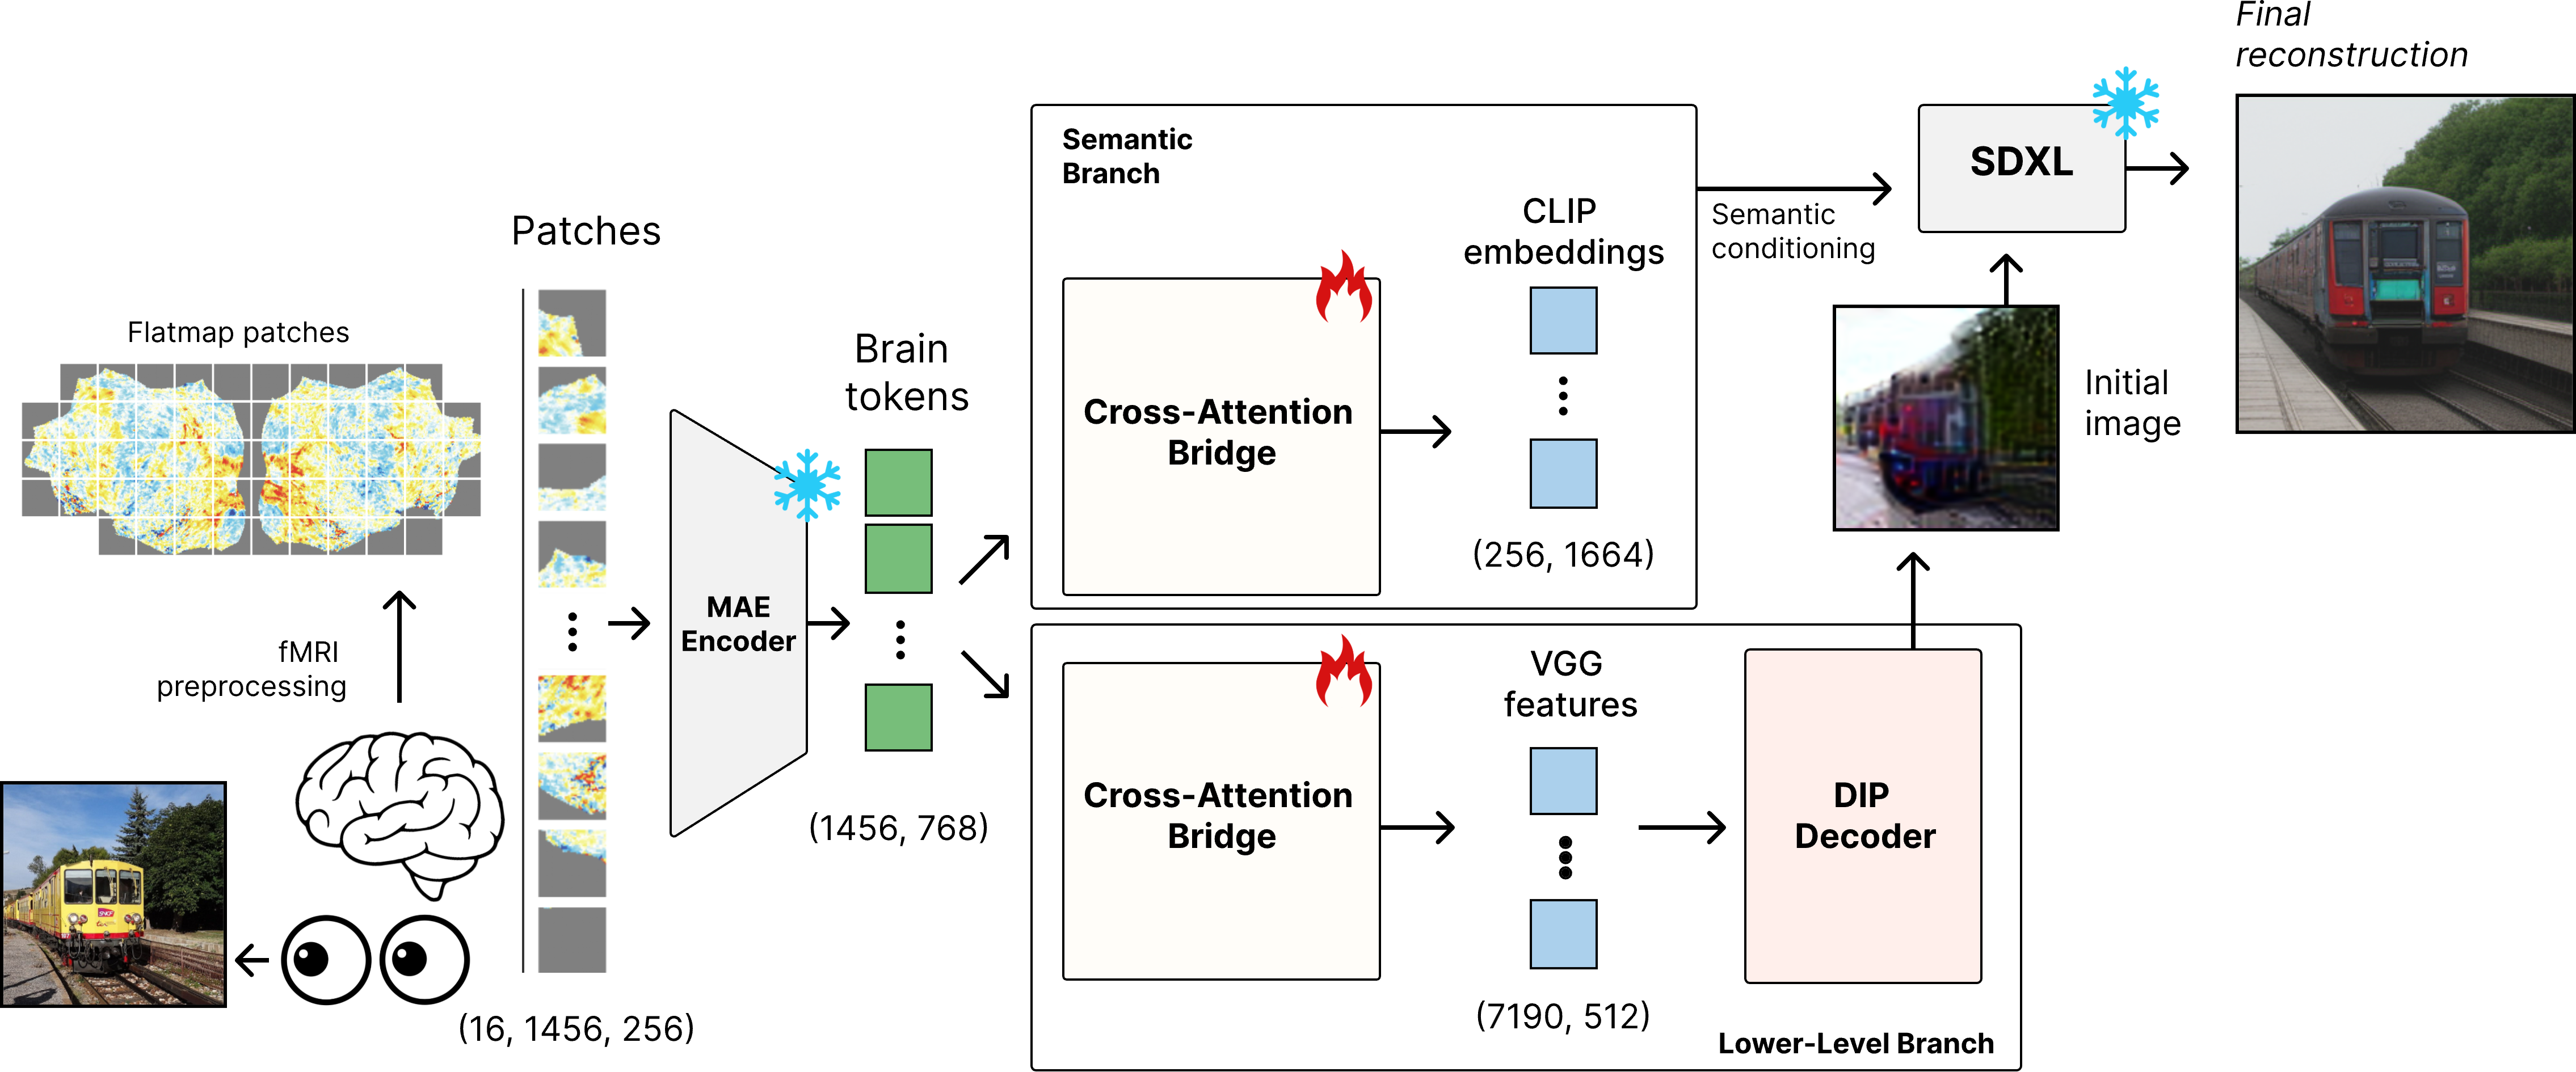
\includegraphics[width=0.75\textwidth]{images/model4.png}
\caption{CortexDecoder overall schematic. From the left side, single-trial betas are projected into 2D cortical flatmaps, then divided into patches. The patches are then encoded by the frozen CortexMAE encoder into 1456 brain tokens, each token having 768 dimensions. The cross-attention bridges, the only trained components, map these tokens into two representation, one for each branch. The semantic branch predicts 256 unpooled OpenCLIP ViT-bigG/14 tokens used as conditioning for a frozen SDXL-unCLIP decoder. The lower-level branch predicts 7190 VGG16-BN feature tokens, which a Deep Image Prior \cite{Ulyanov_2020} decoder inverts into an initial image which encodes for layout, structure of objects and color. Finally a SDXL-unCLIP model takes the initial image and semantic embedding for conditioning to generate the final reconstructed image. Images including those depicting faces are derived from the Microsoft COCO dataset, used under CC BY 4.0. \cite{lin2015microsoftcococommonobjects}}
\label{fig:model_schematic}
\end{figure*}

\section{CortexDecoder}
CortexDecoder is a two-branch brain decoding framework that maps cortical flatmaps representations to high-level semantic and low-level visual features for image reconstruction. The model first encodes cortical flatmaps using a pretrained CortexMAE encoder, producing spatially organized brain tokens. These brain tokens are then fed into the cross-attention bridge which predicts visual image features. The semantic branch predicts unpooled CLIP embedding, while the low-level branch predicts VGG features. Finally, the predicted visual representations are provided to a frozen diffusion decoder to reconstruct the corresponding image.

All model training and evaluations were performed on a single NVIDIA H100 GPU (80 GB). Both branches were trained separately with AdamW \cite{loshchilov2019decoupledweightdecayregularization} (learning rate 5e-4, weight decay 1e-2) and a batch size of 128 under bfloat16 mixed precision. The semantic branch was trained for 25 epochs and the low-level branch also for 25. Deep Image Prior inversion at inference uses 2,000 Adam steps per image with 36 images optimized in parallel for GPU.

\subsection{Natural Scenes Dataset}

The Natural Scenes Dataset (NSD) is a large scale 7T fMRI dataset in which eight participants viewed natural images drawn from MS-COCO (Microsoft Common Objects in Context) \cite{lin2015microsoftcococommonobjects} across up to 40 scan sessions each. Each session comprises 750 trials, each trial presents one image for 3 seconds followed by a 1 second blank. Each subject viewed 10,000 unique images, each repeated 3 times, for a total of 30,000 trials per subject. A subset of 1000 images (shared1000) was presented to all subjects and is reserved as a standard testing set throughout the literature.
NSD employs a rapid event-related design in which new image stimuli are presented every 4 seconds, such that successive stimuli occur within the timescale of . Because of these successive trials overlapping, single-trials cannot be read directly from timeseries. The GLM performs this deconvolution, and its output is a stati   c spatial map of cortical activity per trial rather than a time series. This is precisely the form that 2D flatmap representations and patch-based tokenization assume. We note that the CortexMAE encoder is spatiotemporal and retains a temporal patch dimension from its pretraining on the BOLD time series. However, because our inputs are static single-trial beta maps, we do not utilize this temporal dimension in CortexDecoder.

\subsection{MAE Encoder and Tokenization}
NSD’s surface betas are distributed on a fsaverage mesh (163,842 vertices per hemisphere). We resample them to fsLR-32k (32,492 vertices per hemisphere, 64,984 total), the standard HCP (Human Connectome Project) mesh on which CortexMAE was pretrained. A pycortex-based \cite{DBLP:journals/fini/GaoHLG15} flat-surface resampler then projects these vertices onto a single-channel 224x560 raster resulting in the 2D cortical flatmap. Since the projection is defined by a common template mesh rather than by individual anatomy, a given location in the raster corresponds to approximately the same piece of cortex across subjects.
The flatmap is divided into non-overlapping 16x16 spatial patches, forming a 14x35 grid of 490 cells. Since the cortical surface occupies only part of the bounding box, 364 cells contain cortex and the remaining cells are background. CortexMAE uses a validity mask to exclude these background patches, so only 364 cortical patches are embedded.
CortexMAE is a spatiotemporal masked autoencoder pretrained on BOLD timeseries. In other words, its patching embedding operates over both spaces. For our case, the input is a single-trial beta map, which has no temporal component. To use the pretrained model, we represent each beta map as a static collection of 16-frames. Since we use CortexMAE encoder out of the box, we also retain its output shape, a sequence of 1456 tokens each with a dimension of 768.

\begin{figure}[!t]
\centering
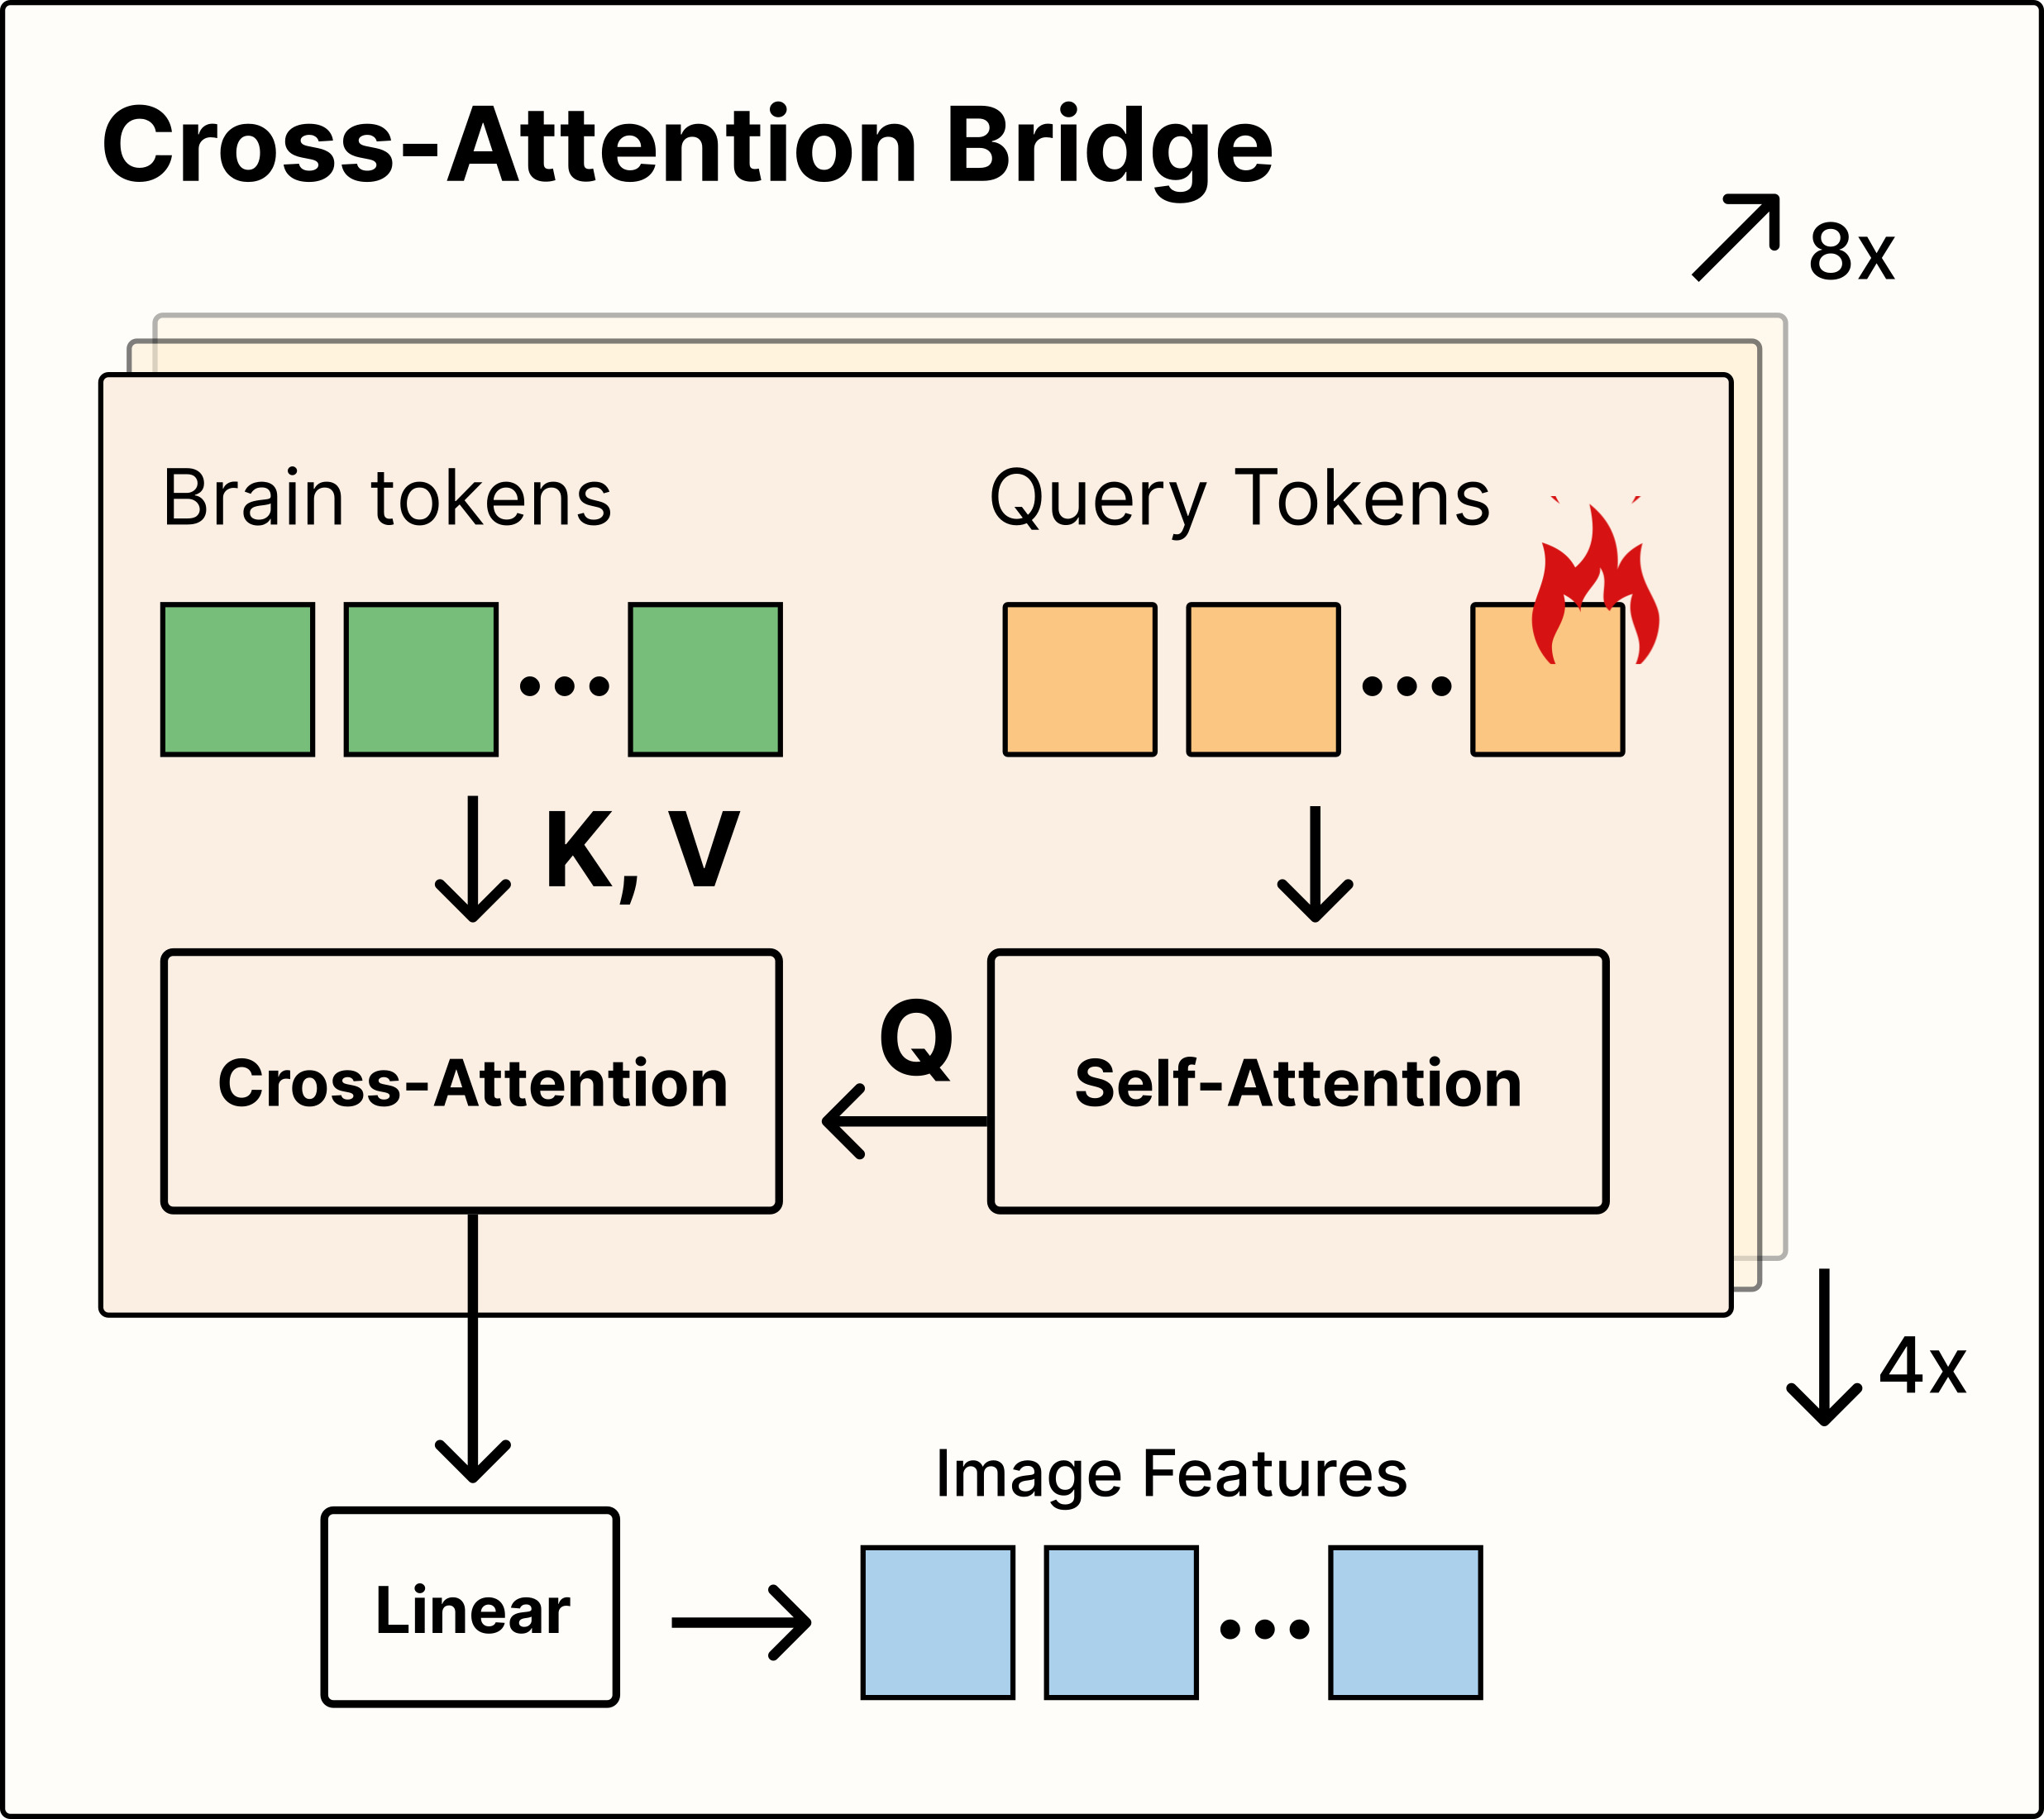
\includegraphics[width=0.8\columnwidth]{images/cross.jpg}
\caption{Cross-attention bridge. The brain tokens supply key and values while learned query tokens serve as queries. There is one learned query token for each output feature token. Each attention block first applies self attention among query tokens, followed by a cross-attention from queries to brain tokens. We have 8 attention heads followed by a FFN. There are 4 layers of multi-head attention blocks with a subsequent linear projection to match the shape of the image features. A separate bridge is instantiated for each branch, with the number of query tokens and output dimensionality determined by the target. Images including those depicting faces were derived from the Microsoft COCO dataset, used under CC BY 4.0. \cite{lin2015microsoftcococommonobjects}}
\label{fig:cross_attention_bridge}
\end{figure}

\subsection{Cross-Attention Bridge}
The bridge maps the sequence of brain tokens to a sequence of visual feature tokens. Its design follows DETR (DEtection TRansformer) \cite{DBLP:journals/corr/abs-2005-12872}. We define a set of learned query vectors with one query per output token. These are randomly initialized and trained jointly with the rest of the model. Each query is responsible for predicting one token of the target visual representation.
The brain tokens serve as memory. They are layer-normalized and project to the model width when the two dimensions differ. In our case, CortexMAE embedding dimension and the bridge width are both 768 so no projection is needed. The queries are then passed through a stack of transformer decoder layers. Each layer applies self-attention among the queries then cross-attention from the queries into the brain memory then a position wise feed-forward network (FFN). Self-attention lets the queries coordinate with one another so that neighboring output tokens can share information. Cross-attention is where the decoding happens. Each query attends over all 1456 brain tokens and pools the ones that carry information about its target feature. A final linear layer projects each decoded query to the dimensionality of the target representation.
We use a 4 decoder layer and 8 attention heads. The model width is 768 with a feed-forward dimension of 3072 and dropout of 0.1. Both semantic and lower-level branches share these settings.
The key property of this design is that the brain representation remains a sequence throughout. Each query attends over the full set of brain tokens. A pooled brain vector would make every query attend to the same input and reduce the decoder to a multilayer perceptron (MLP) applied identically at each output position.

We instantiate the bridge twice with one instance per branch and train the two independently rather than sharing a trunk. The semantic branch uses 256 queries and projects to 1664 dimensions. This matches the shape of the unpooled OpenCLIP ViT-bigG/14 \cite{radford2021learningtransferablevisualmodels, ilharco_gabriel_2021_5143773, schuhmann2022laionb} patch tokens that the diffusion decoder expects as conditioning. The low-level branch uses 7190 queries and projects to 512 dimensions. This matches the concatenated token count of the five VGG16-BN feature layers described in section 3.6. The two branches therefore differ by more than an order of magnitude in output length. They also optimized different losses, since the semantic target is dense and continuous while the low-level target is better matched by contrastive objective.

% TODO: We need to validate the loss functions here.

\begin{equation}
\mathcal{L}_{\mathrm{CLIP}} = \mathrm{MSE}\big(\hat{\mathbf{C}}, \mathbf{C}\big),
\end{equation}

\medskip

where $\hat{\mathbf{C}}, \mathbf{C} \in \mathbb{R}^{256 \times 1664}$ are the predicted and target OpenCLIP token sequences, averaged over all tokens, dimensions and images in the batch.

\begin{equation}
\mathcal{L}_{\mathrm{VGG}} = \frac{1}{5}\sum_{l=1}^{5} \mathcal{L}_{\mathrm{NCE}}\big(\hat{\mathbf{z}}^{(l)}, \mathbf{z}^{(l)}\big),
\end{equation}

\medskip

% where $\mathcal{L}_{\mathrm{NCE}}$ is a symmetric InfoNCE loss with temperature $\tau = 0.07$ computed independently at each sampled token position of VGG layer $l$: the predicted and target tokens from the same image form the positive pair, and tokens from the other images in the batch serve as negatives. Similarities are cosine, and the loss is averaged over positions.


The low-level branch is trained with a symmetric position-wise contrastive loss over sampled VGG feature tokens. This is an InfoNCE-style \cite{oord2019representationlearningcontrastivepredictive} objective, where for each sampled token position, the positive pair is the predicted and target VGG token from the same image, while the negatives are the corresponding target tokens from other images in the batch. Contrastive loss is used instead of MSE as it can reward averaged feature predictions, which could end up in blurry predictions. But contrastive loss instead trains the model to distinguish between one image’s VGG features over another image, making the predicted features more image-specific.



\subsection{Semantic Branch}
The semantic branch predicts the image representations that conditions the diffusion decoder. Its target is the unpooled patch tokens sequence produced by the OpenCLIP ViT-bigG/14 vision encoder pretrained on LAION-2B \cite{schuhmann2022laionb}. For each stimulus image we take the 256 patch tokens before the final projection and discard the class token (referred to as CLS token). Each token is 1664 dimensional. The bridge therefore uses 256 queries and projects to 1664 dimensions so that its output matches the target.

We use an unpooled token sequence rather than a single pooled embedding. A pooled CLIP vector summarizes an image but discards where its content sits in the frame. A token sequence retains that layout and gives the diffusion decoder a spatially structured condition signal. The diffusion decoder we use is a pretrained SDXL-unCLIP model whose cross-attention was trained to condition on exactly 256 bigG tokens of 1664 dimensions. Matching this shape means the decoder can be used frozen with no fine-tuning on our part. Predicting a smaller CLIP variant would require retraining the decoder’s conditioning pathway.

The OpenCLIP encoder is frozen and used only to produce targets. We extract the token sequence for every stimulus image once and cache it. During training, the branch never runs the image encoder. The branch is trained with mean squared error between the predicted and target token sequences, averaged over all 256 positions and 1664 dimensions.

\begin{figure}[!t]
\centering
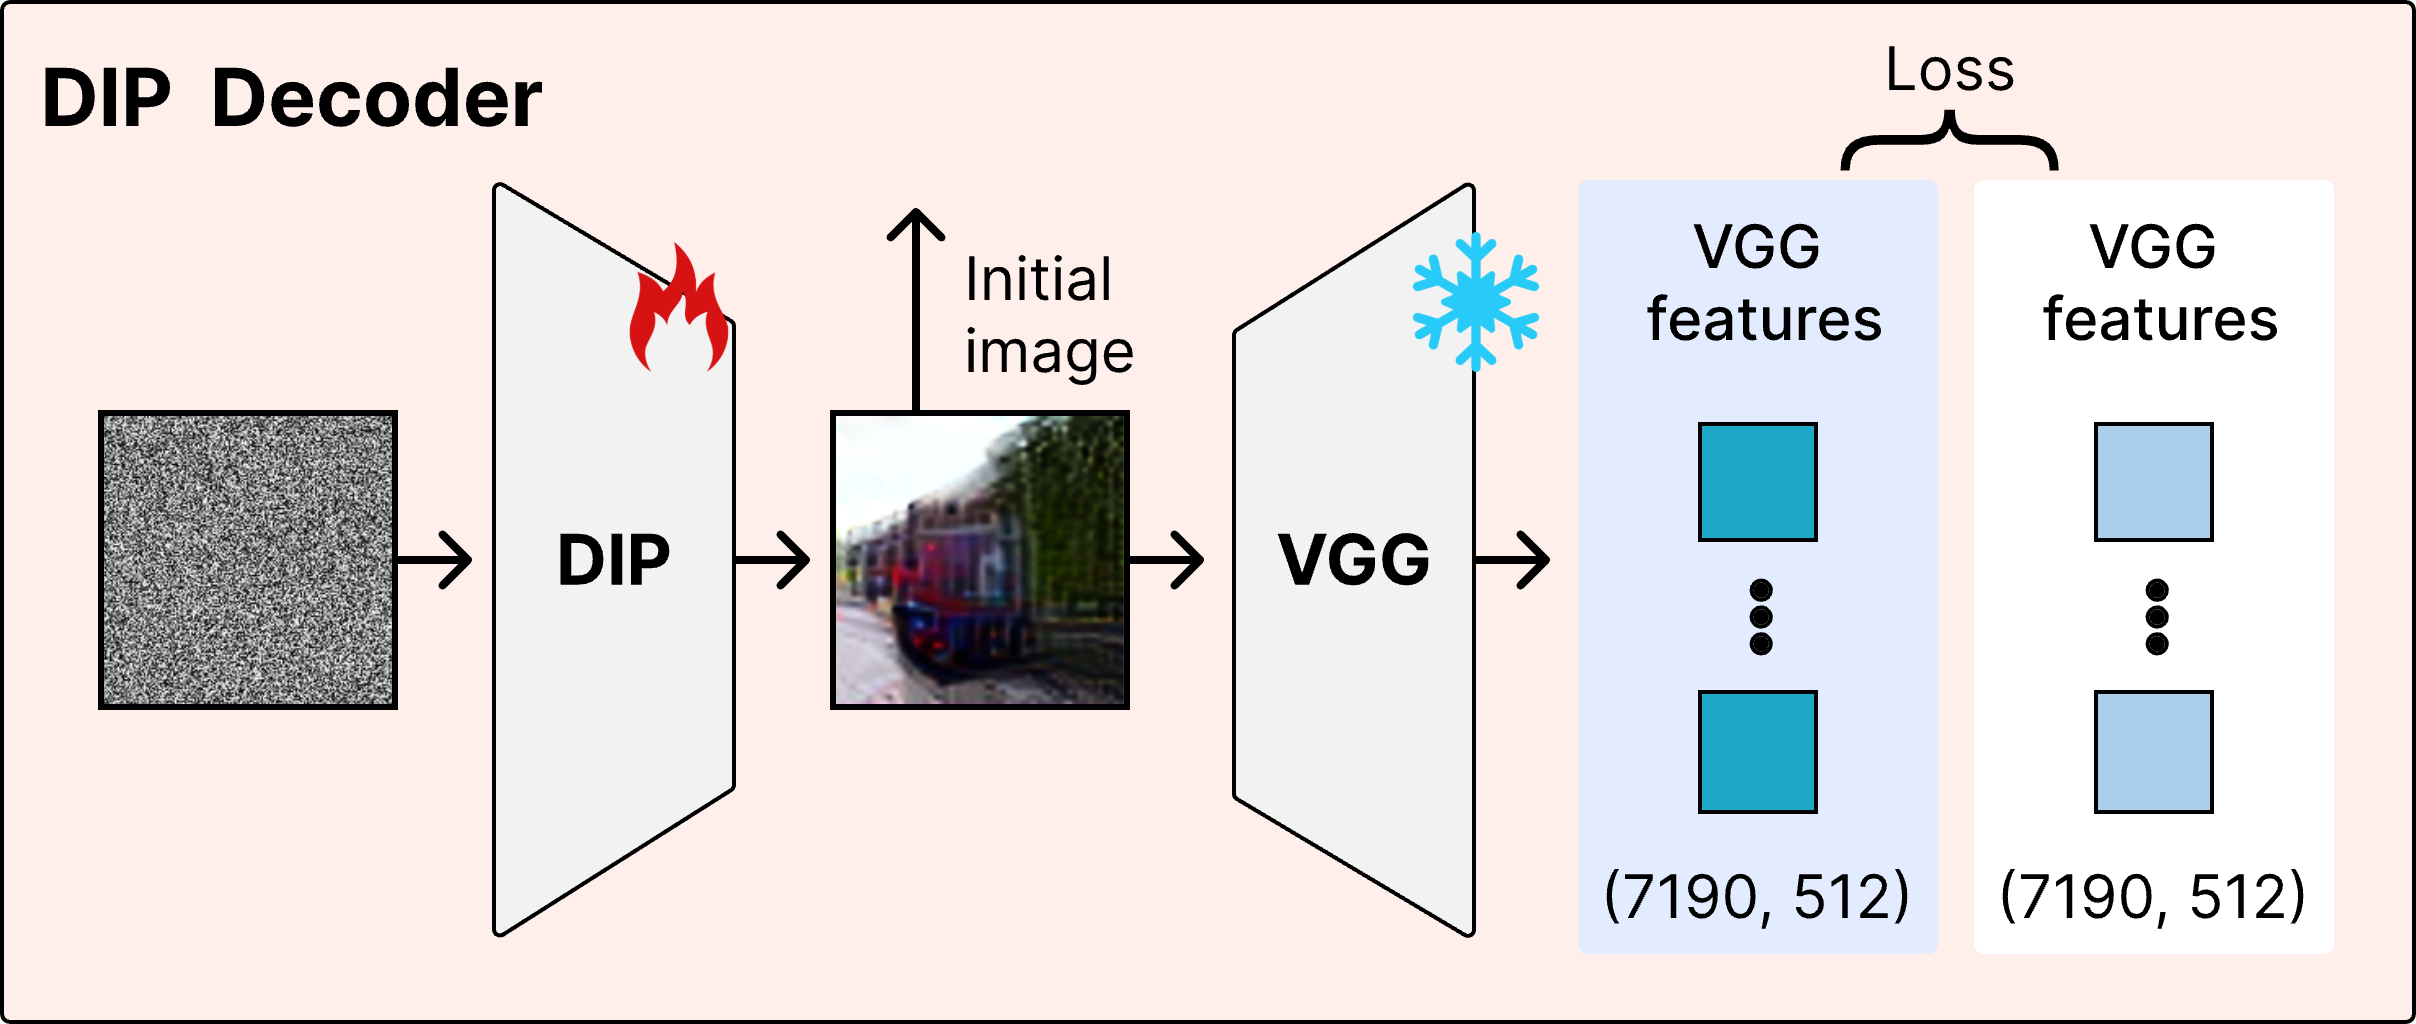
\includegraphics[width=1\columnwidth]{images/DIP3.png}
\caption{Low-level image reconstruction from predicted VGG16-BN feature activations with Deep Image Prior Inversion. We use the DIP U-Net to project random Gaussian noise to an RGB image. The image is passed through a frozen VGG16-BN network, and the output feature activations are compared with the target activations predicted by the Cross-Attention Bridge model. The DIP U-Net is optimized with 2000 training steps, and its output becomes the final low-level image reconstruction.}
\label{fig:dip_reconstruction}
\end{figure}

\subsection{Low-Level Branch}
With the predicted VGG feature representation, we reconstruct a low-level image through Deep Image Prior inversion. The predicted VGG representation is not a single output embedding, but the last five convolutional activation layers of the VGG16-BN image model.

To convert this representation into pixels, we optimize a Deep Image Prior U-Net per low-level image inference.  It is a small encoder-decoder convolutional generator, which maps random Gaussian noise to an RGB image, and the image is subsequently passed through a frozen VGG16-BN network.

Then the extracted VGG feature representation is compared against the brain-predicted VGG representation using MSE loss. The gradient is backpropagated through only the DIP U-Net, iteratively updating the generator for a fixed 2000 optimization steps to produce the final low-level reconstruction.

\subsection{Final Image Reconstruction}
To generate the final image reconstruction, we combine the low-level DIP image with the semantic CLIP prediction using the MindEye2 Standard Diffusion unCLIP model (SDXL-unCLIP). The SDXL-unCLIP is a pretrained image generation model that reconstructs images from OpenCLIP ViT-bigG/14 embeddings, instead of embedded text prompts. The intention is for the low-level DIP image to provide layout, color, and coarse structure while the predicted OpenCLIP ViT-bigG/14 tokens determine semantic context of the image.

We first add gaussian noise to the low-level image to partially corrupt fine detail while preserving coarse layout/color. This re-noised image becomes the initialization state for Standard Diffusion unCLIP model, anchoring the image structure. The predicted OpenCLIP token representation subsequently conditions the denoising process towards the correct semantic context, turning the blurred low-level reconstruction into a detailed final image. Using this approach, the reconstruction should accurately reflect the content of the image and the structure. We run this diffusion process multiple times for each image and select the final reconstruction whose down-scaled version has the lowest MSE relative to the low-level reconstruction. This encourages the final diffused image to not stray too far from the predicted low-level image structure.

\begin{figure}[!b]
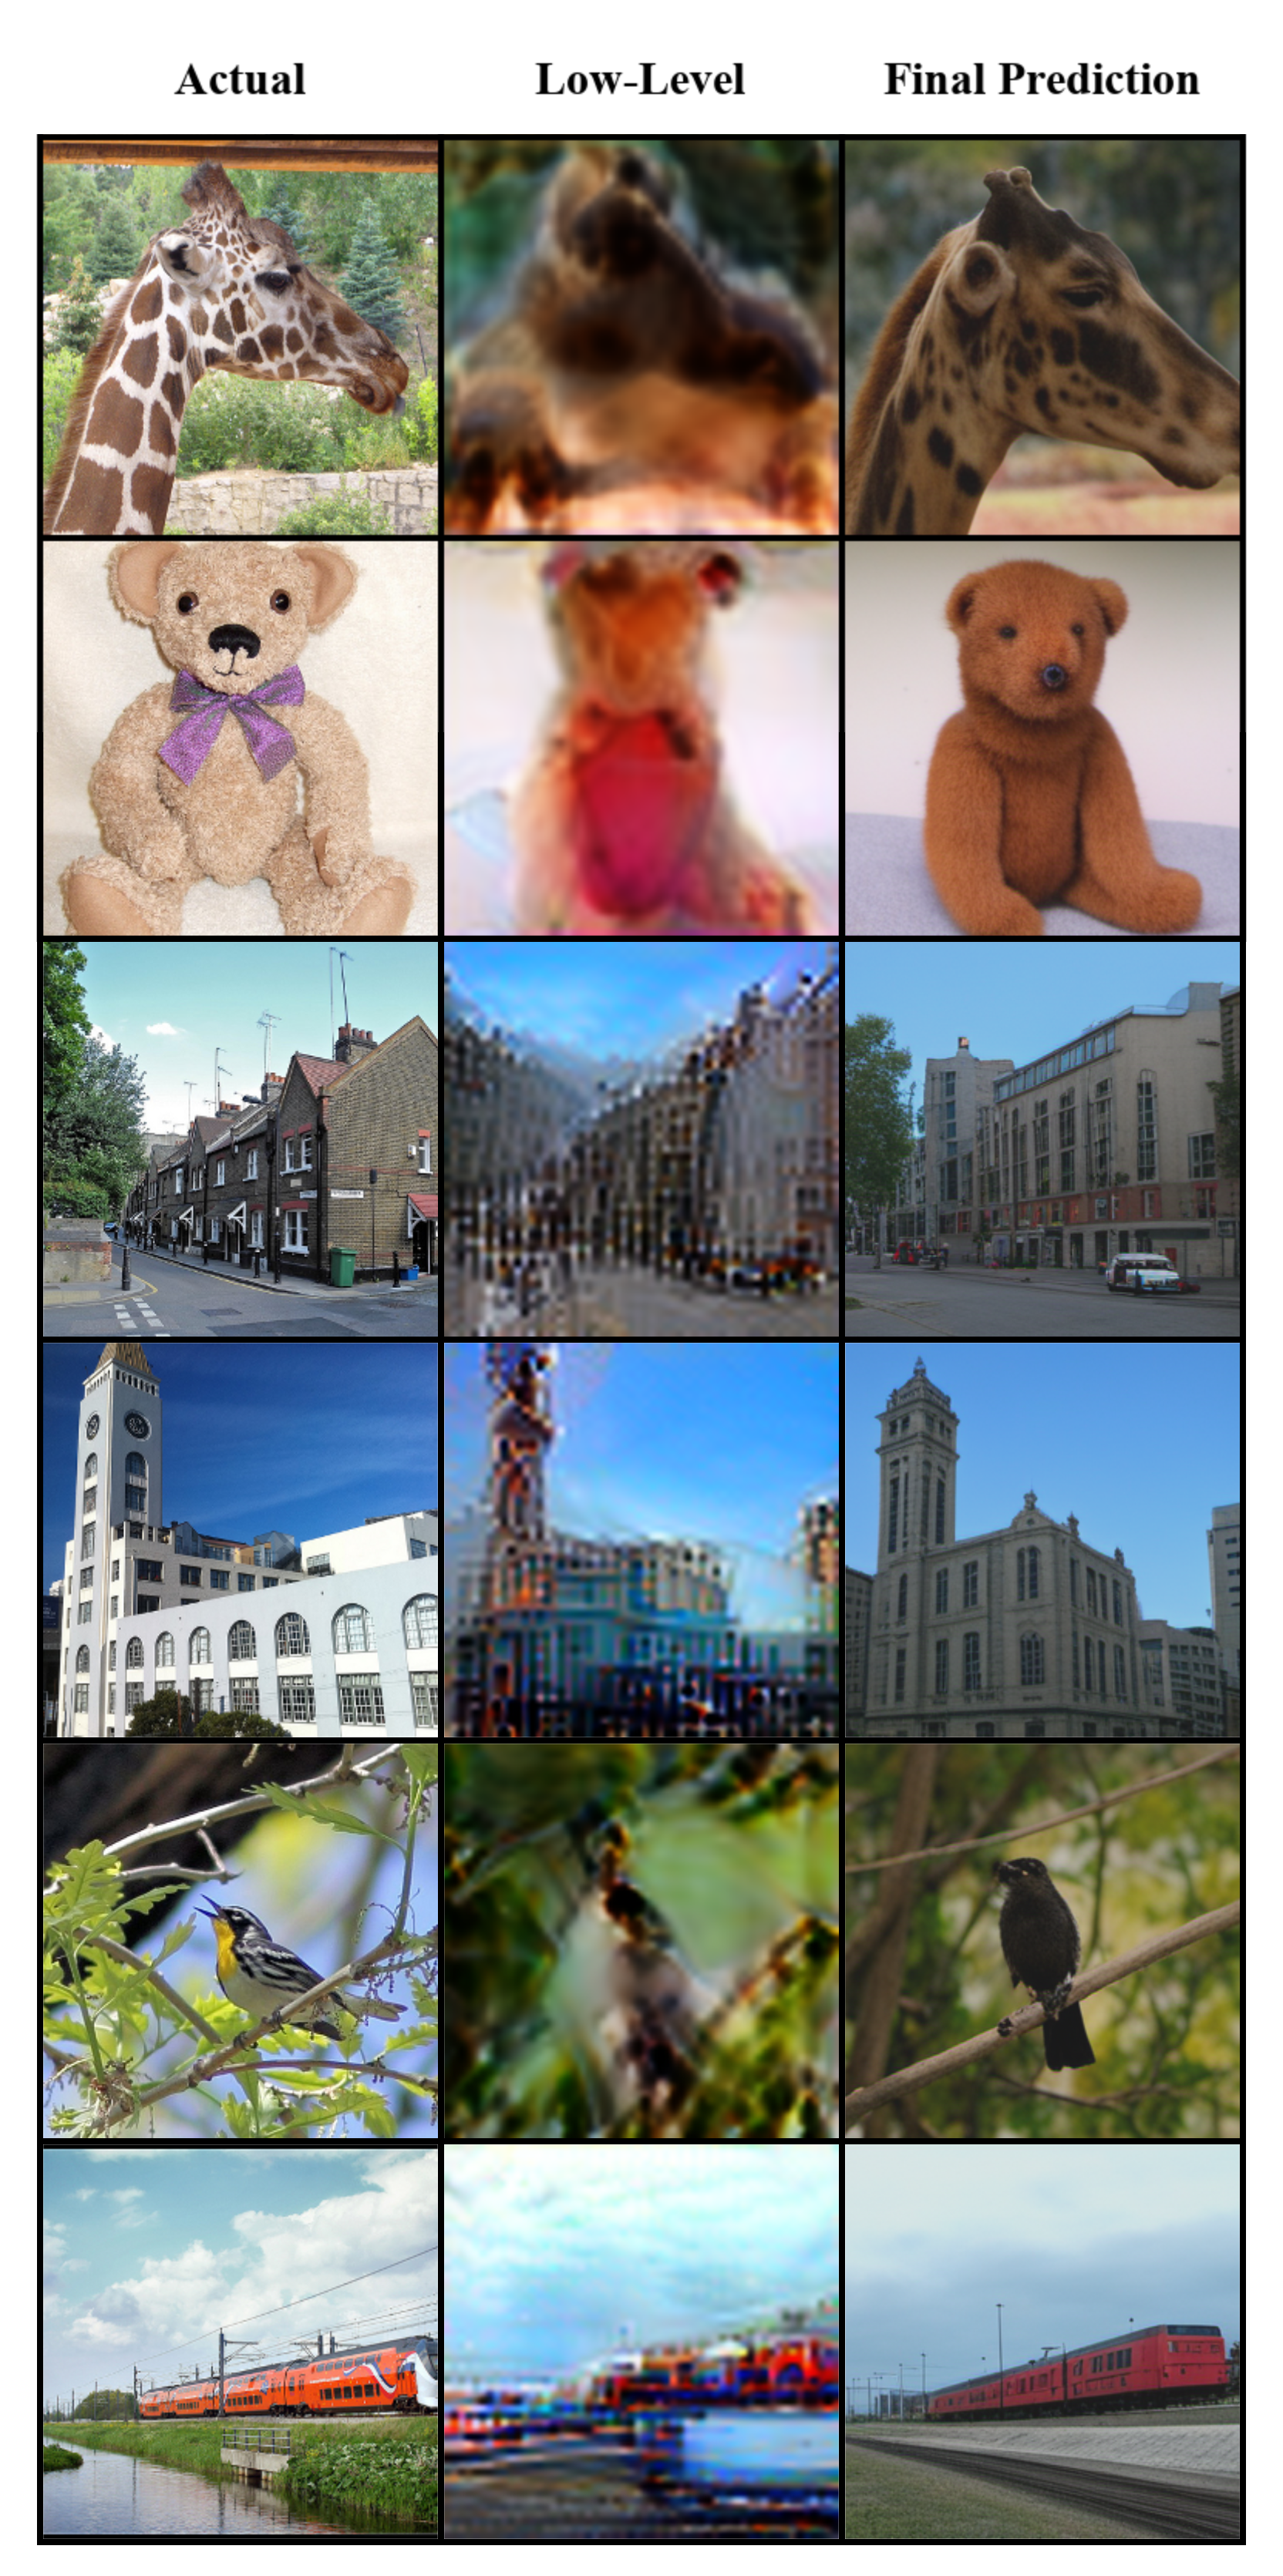
\includegraphics[width=0.65\columnwidth]{images/stacked_triptych_collage2.png}
\centering
\caption{Comparing low-level reconstruction (middle column) with final reconstruction (rightmost column). The left column is the original COCO image stimulus. Each row shows different types of reconstructions of the original image stimulus. Images including those depicting faces are derived from the Microsoft COCO dataset, used under CC BY 4.0. \cite{lin2015microsoftcococommonobjects}}
\label{fig:stacked_triptych}
\end{figure}

\section{Results}
We evaluate CortexDecoder in the shared1000 from the NSD, a dataset completely separated from training and validation to prevent leakage. All metrics computed compare reconstruction against the stimulus images viewed by subject one. We report, PixCorr (Pixel Correlation), SSIM (Structural Similarity Index Measure) \cite{1284395}, AlexNet(2), AlexNet(5) \cite{NIPS2012_c399862d}, InceptionV3 \cite{szegedy2015rethinkinginceptionarchitecturecomputer}, CLIP \cite{radford2021learningtransferablevisualmodels}, EfficientNet-B1 \cite{tan2020efficientnetrethinkingmodelscaling} and SwAV-ResNet50 \cite{caron2021unsupervisedlearningvisualfeatures}. PixCorr and SSIM measure pixel and structural similarity while AlexNet, InceptionV3, CLIP measure feature space similarity. EfficientNet and SwAV report correlation distance, where lower is better.

We report both the lower-level DIP reconstruction and the final diffusion reconstruction. This isolates the contribution of the semantic branch and the diffusion stage beyond the structural information recovered by the lower-level branch. Because diffusion is stochastic, we generate 20 candidates per image. Then we select the generated image with the lowest pixelwise MSE to the low-level reconstruction after resizing. This approach does not use ground-truth images and favors candidates that preserve the predicted structure.

\subsection{Reconstruction Benchmarks}
Overall, CortexDecoder is competitive with low-level and mid-level features while we report weaker results in terms of semantics. Specifically, our model performs well for PixCorr and SSIM reflecting the contribution of the lower-level branch.

From the results it is clear that the introduction semantic conditioning negatively impacts the modeling of lower level features. For example, the low-level method on its own scores higher on the low-level benchmarks compared to the samples where semantic conditioning was introduced in the diffusion stage. We conclude that the final reconstruction which takes into account both semantic and low-level representation improves on semantic metrics at the expense of low-level performance.

\begin{table*}[!t]
\centering
\footnotesize
\renewcommand{\arraystretch}{1.25}
\setlength{\tabcolsep}{5pt}
\begin{tabular*}{\textwidth}{@{\extracolsep{\fill}}lcccccccc}
\toprule
& \multicolumn{4}{c}{Low-Level}
& \multicolumn{4}{c}{High-Level} \\
\cmidrule(lr){2-5}\cmidrule(lr){6-9}
\textbf{Method}
& PixCorr $\uparrow$
& SSIM $\uparrow$
& Alex(2) $\uparrow$
& Alex(5) $\uparrow$
& Incep $\uparrow$
& CLIP $\uparrow$
& Eff $\downarrow$
& SwAV $\downarrow$ \\
\midrule
% \textit{Takagi \& Nishimoto (2023) \cite{10205187}}
% & 0.239 & 0.377 & 78.47\% & 85.52\%
% & 83.24\% & 82.64\% & 0.817 & 0.510 \\
\textit{Brain-Diffuser \cite{ozcelik2023brain}}
& 0.305 & 0.367 & 96.7\% & 97.4\%
& 87.8\% & 92.5\% & 0.768 & 0.415 \\
\textit{MindEye \cite{scotti2023reconstructingmindseyefmritoimage}}
& \textbf{0.390} & 0.337 & 97.4\% & 98.7\%
& 94.5\% & 94.6\% & 0.630 & 0.358 \\
\textit{DREAM \cite{xia2024dreamvisualdecodingreversing}}
& 0.288 & 0.338 & 95.0\% & 97.5\%
& 94.8\% & \underline{95.2\%} & 0.638 & 0.413 \\
\textit{MindEye2$^\dagger$ \cite{scotti2024mindeye2sharedsubjectmodelsenable}}
& 0.374 & \textbf{0.439} & 97.8\% & 99.1\%
& \underline{96.2\%} & 93.6\% & \underline{0.609} & 0.338 \\
\textit{NeuroPictor$^\dagger$ \cite{huo2024neuropictorrefiningfmritoimagereconstruction}}
& 0.277 & 0.385 & \textbf{98.8\%} & \underline{99.3\%}
& \underline{96.2\%} & 94.5\% & 0.619 & \underline{0.334} \\
\textit{UMBRAE$^\dagger$ \cite{xia2024umbraeunifiedmultimodalbrain}}
& 0.293 & 0.345 & 95.8\% & 97.2\%
& 92.6\% & 93.9\% & 0.690 & 0.391 \\
\textit{MindTuner$^\dagger$ \cite{gong2024mindtunercrosssubjectvisualdecoding}}
& 0.371 & \underline{0.428} & 97.7\% & \underline{99.3\%}
& \textbf{96.4\%} & 94.3\% & \textbf{0.601} & \textbf{0.331} \\
\textit{NeuralDiffuser \cite{Li_2025}}
& \underline{0.378} & 0.330 & \underline{98.3\%} & \textbf{99.4\%}
& 95.8\% & \textbf{95.4\%} & 0.642 & 0.380 \\
\midrule
\textbf{\textit{CortexDecoder (Ours)} - Low-Level}
& \textbf{0.390} & 0.407 & 97.6\% & 99.2\%
& 90.9\% & 75.9\% & 0.845 & 0.580 \\
\textbf{\textit{CortexDecoder (Ours)} - Final}
& 0.370 & 0.414 & 96.6\% & 97.7\%
& 92.5\% & 91.4\% & 0.675 & 0.385 \\
\bottomrule
\end{tabular*}
\caption{Quantitative comparison of CortexDecoder with existing fMRI-to-Image reconstruction methods on the NSD shared1000 test set for Subject 1. We report the performance for both the low-level reconstruction produced from the predicted VGG features using Deep Image Prior (DIP) and the final diffusion reconstruction conditioned on the predicted semantic and low-level representations. PixCorr denotes pixelwise correlation and SSIM denotes structural similarity. AlexNet(2), AlexNet(5), InceptionV3, CLIP, EfficientNet-B1 (Eff), and SwAV-ResNet50 (SwAV) measure similarity in learned feature spaces. EfficientNet and SwAV are reported as correlation distance, where lower is better. \textbf{Bold} indicates the best performance and \underline{underline} indicates the second best performance. All baseline values are the Subject 1 results reported by the respective papers. $^\dagger$ denotes methods that pretrain on multiple subjects before subject-specific fine-tuning (UMBRAE is a single cross-subject model evaluated on Subject 1).}
\label{tab:subject1_reconstruction}
\end{table*}


\section{Conclusion}
We introduce CortexDecoder, an fMRI-to-image reconstruction framework that uses 2D cortical flatmaps as neural representations for visual decoding. Converting cortical flatmaps into token patches, CortexDecoder enables use of Vision Transformers while preserving the spatial component of cortical responses. A pretrained CortexMAE encoder produces brain tokens, which are then mapped through a dual cross-attention branch; one semantic and another for low-level image reconstruction. These representations are then combined with a finetuned SDXL-unCLIP, taking the predicted low-level image as an initial image and conditioning on the predicted semantic embedding to produce the final reconstruction image.
Our results show that cortical flatmaps preserve enough information to support brain decoding. CortexDecoder excels at low level reconstruction particularly with the PixCorr and SSIM evaluation metrics for a single subject. Overall, flatmaps are promising as an fMRI representation for brain decoding, specifically as we’ve demonstrated for image reconstruction tasks.

\section{Limitations}
Due to compute and budget constraints, our experiments are isolated to NSD subject 1, instead of the full four-subject evaluation used in the aforementioned prior works. We therefore only compare against subject-1 results from other works when available, and do not compare against multi-subject averages. A clear direction of future work is to extend our methods across all subjects, and evaluate if the identified patterns of results sustain for all subjects.

Additionally, our compute and budget constraints restricted hyperparameter tuning, design iteration, and repeated full evaluations that would help in optimizing our evaluated metrics. We were only able to perform one full evaluation run, rather than multiple design iterations, which may partially explain the gap to other state-of-the-art models on the high-level metrics.

\section{Future Work}
Our future work will extend our experiments from solely NSD subject 1 to the full four-subject setting which other papers use. This would evaluate whether the observed performance of our pipeline holds up across all subjects with differing brain anatomies.

We would likely implement this by introducing a shared functional clustering space across subjects. Specifically, we would summarize each flatmap patch across trials into a single description vector, then fit a Gaussian Mixture Model \cite{dempster1977maximum} to map brain patches from all subjects into a common cluster space. A cross-attention layer could then compress the patches assigned to each cluster into a fixed set of cluster tokens. Similar strategies have proven effective in prior work for training a single transferable model across many subjects.

Together, these extensions would enable a more direct comparison against prior multi-subject methods and test whether our approach remains competitive at scale.

Another direction is to replace CLIP as the target semantic representation, with an embedding space from more recent model such as SigLIP2 \cite{tschannen2025siglip2multilingualvisionlanguage}. One limitation is that semantic conditioning with the CLIP embeddings comes at the expense of our low-level performance. Replacing CLIP with a stronger semantic embedding model such as SigLIP2 could improve our visual-semantic alignment, and subsequent performance on both low-level and high-level evaluations. This may require training an SDXL decoder that accepts SigLIP2 embeddings as conditioning inputs.

\begin{figure}[!t]
\centering
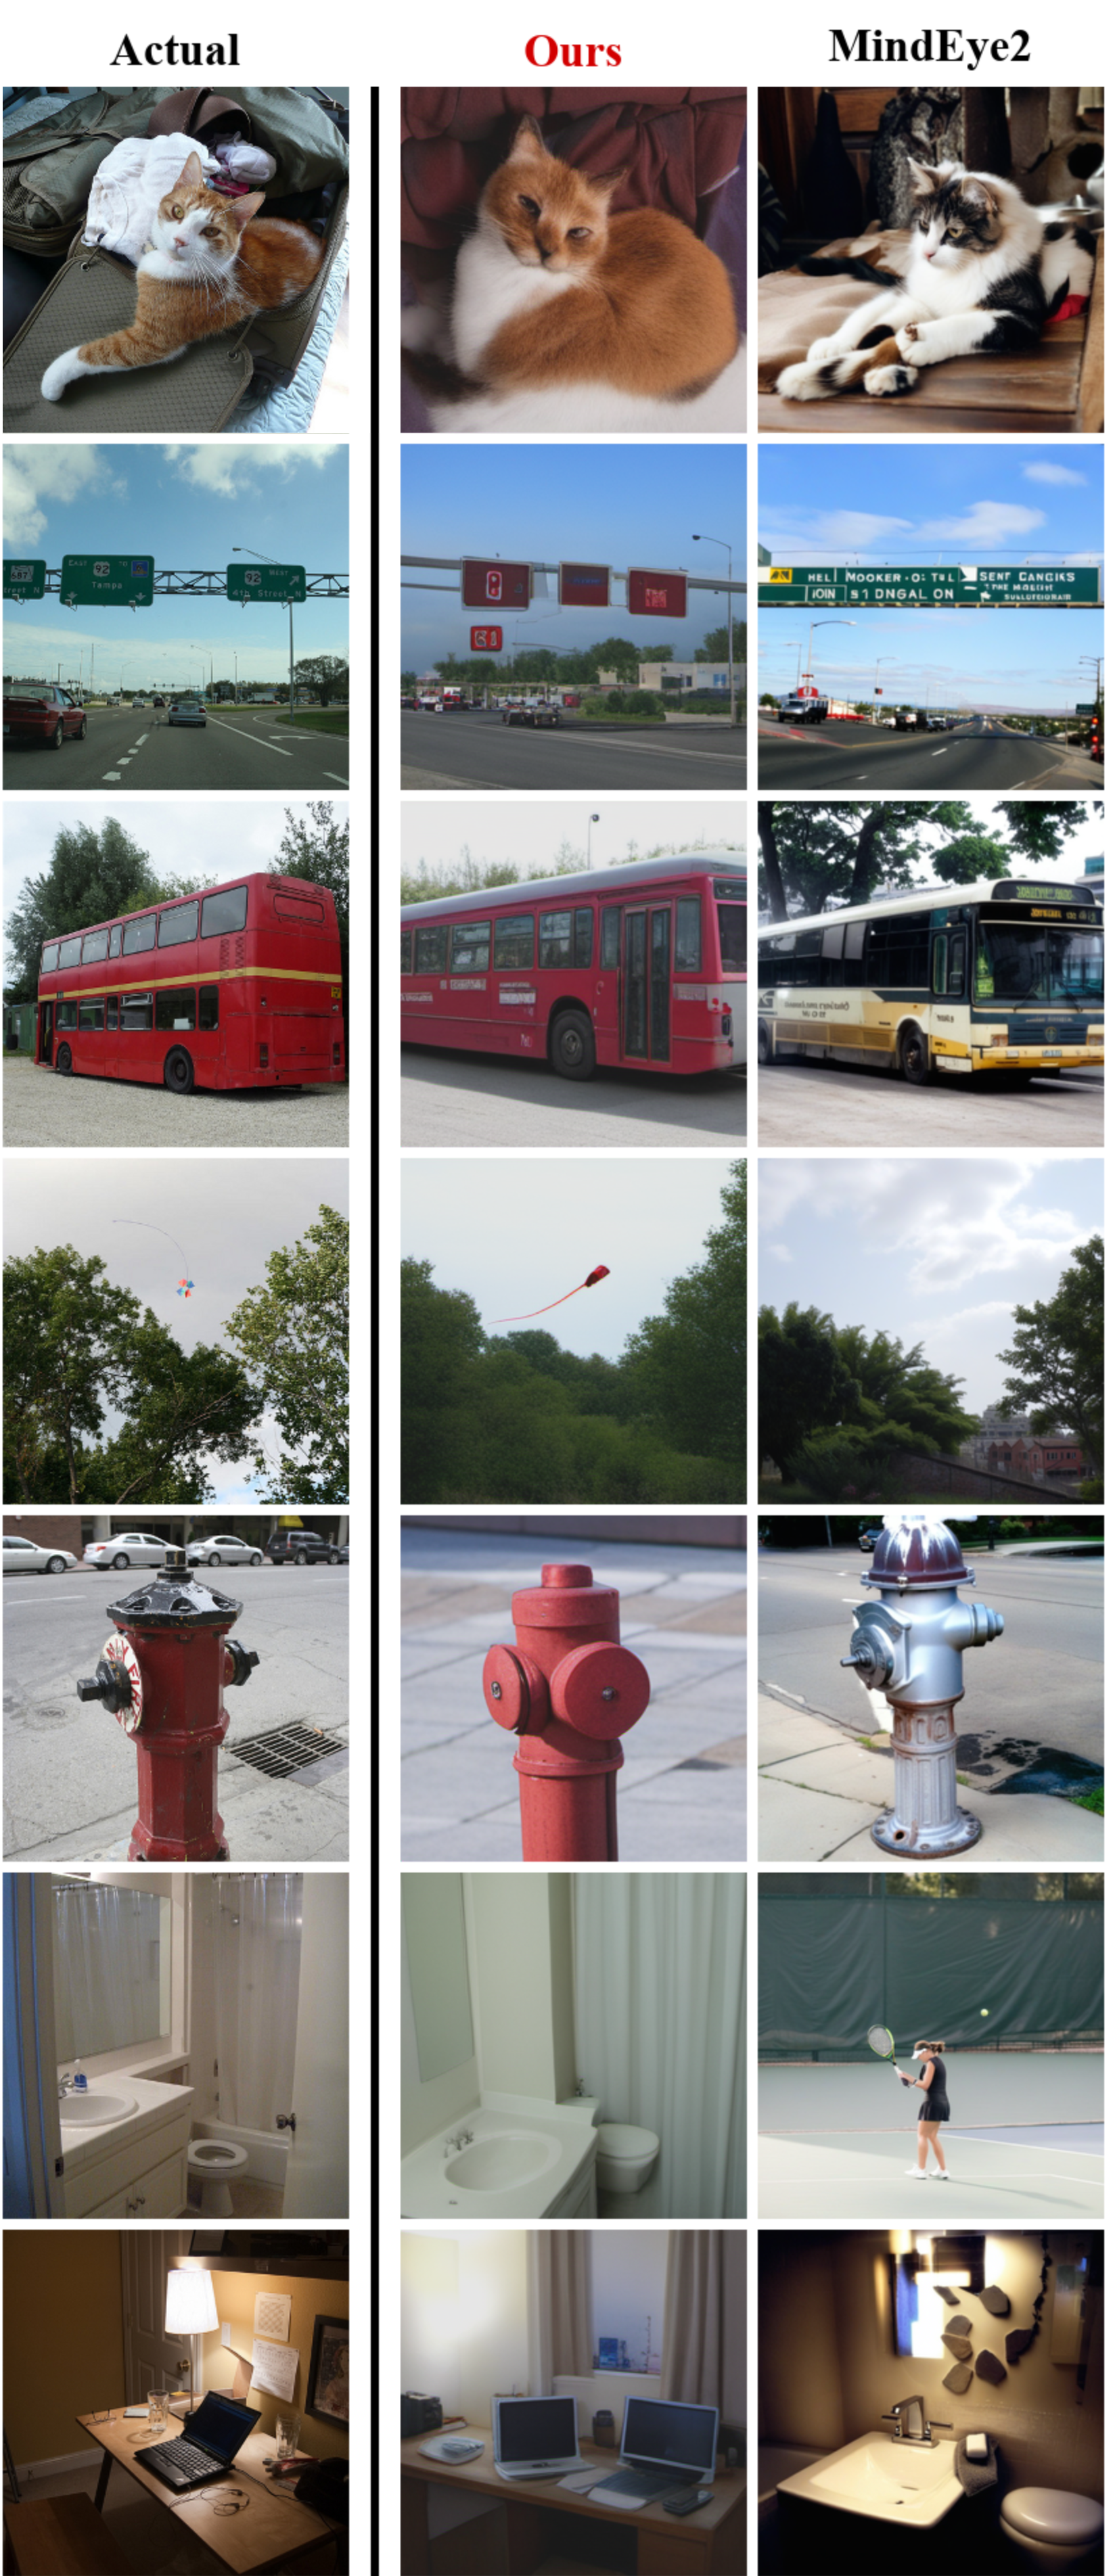
\includegraphics[width=0.8\columnwidth]{images/comparison3.png}
\caption{Image reconstructions comparing models. The left column shows the original image stimuli, middle column is our model, and rightmost column is MindEye2 generations. Each row corresponds to a reconstruction of the same image stimulus. Images including those depicting faces are derived from the Microsoft COCO dataset, used under CC BY 4.0. \cite{lin2015microsoftcococommonobjects}}
\label{fig:comparison}
\end{figure}

% \section*{References}

% \clearpage
\bibliographystyle{abbrv}
\bibliography{references}

\end{document}
